\documentclass[10pt,a4paper]{report}
\usepackage[a4paper,left=20mm,right=20mm,top=25mm,bottom=20mm]{geometry}
\usepackage{amsfonts}
\usepackage{xcolor}
\usepackage{graphicx}
\graphicspath{{./images/}}
\usepackage{csquotes}
\usepackage{hyperref}
\usepackage{listings}
\usepackage{geometry}
\usepackage{float}

\hypersetup{
    colorlinks=true,
    urlcolor=darkgray,
	linkcolor=black
}

\title{\huge{\textbf{Data Mining Project Report}}}
\author{Funaioli Francesca\\
Karoui Hamza\\
Mitola Francesco\\
Vezzuto Samuele\\
}

\begin{document}

\makeatletter
\begin{titlepage}
	\begin{center}
		
\includegraphics[width=0.4\linewidth]{unipi}\\[4ex]
		{\huge \bfseries  \@title }\\[2ex]
		{\Large A.Y. 2023/2024 }\\[6ex]
		{\large  \@author}
	\end{center}
\end{titlepage}
\makeatother

\tableofcontents
\thispagestyle{empty}
\clearpage
\pagenumbering{arabic}
\chapter{Data Understanding}

\section{Datasets Analysis}

The data understanding phase aims to prepare data for the following data mining tasks and to gain informations on the general properties of our data.
This phase of data analysis is focused on an identification of missing values, outliers, duplicates and distribution analysis.
The three csv files, \texttt{incidents.csv}, \texttt{povertyByStateYear.csv} and \texttt{year\_state\_district\_house.csv} were imported and analyzed separately.
The first preliminary checks comprised looking for null values and checking the data types of the attributes, before a more in depth analysis of each column of each dataset.
By computing the statistics of the numerical values of each dataset, we noticed a wrong value in attribute \textit{participant\_age\_1} (values of 311).
We also found out that some of the columns considered contained non-numerical values, as they were not displayed when the pandas \texttt{describe()} method was used.
The value of 0 for attribute \textit{participant\_age\_1} occurs when there are infants involved and therefore it is not to be considered a wrong value.
In a similar way, \textit{n\_participants} has value 0 if the incident had no victims or no shots where fired, but also in records with most of the attributes set to null.

\subsection{Incidents}

\subsubsection{Date}

Each \textit{date} value was converted to a datetime object, after checking that there where no null or NaT values.
The plot in Figure \ref{incidents_per_year}, representing the number of incidents per year, shows an increasing trend in the number of crimes over the years.
It also shows a lack of records related to years 2013 and 2018: there are only 253 incidents happened in 2013, hence they will be removed during data preparation.
As for the year 2018, there is only data relating to the first three months of the year in the dataset, so year 2018 will be analyzed on its own.

\begin{figure}[h]
	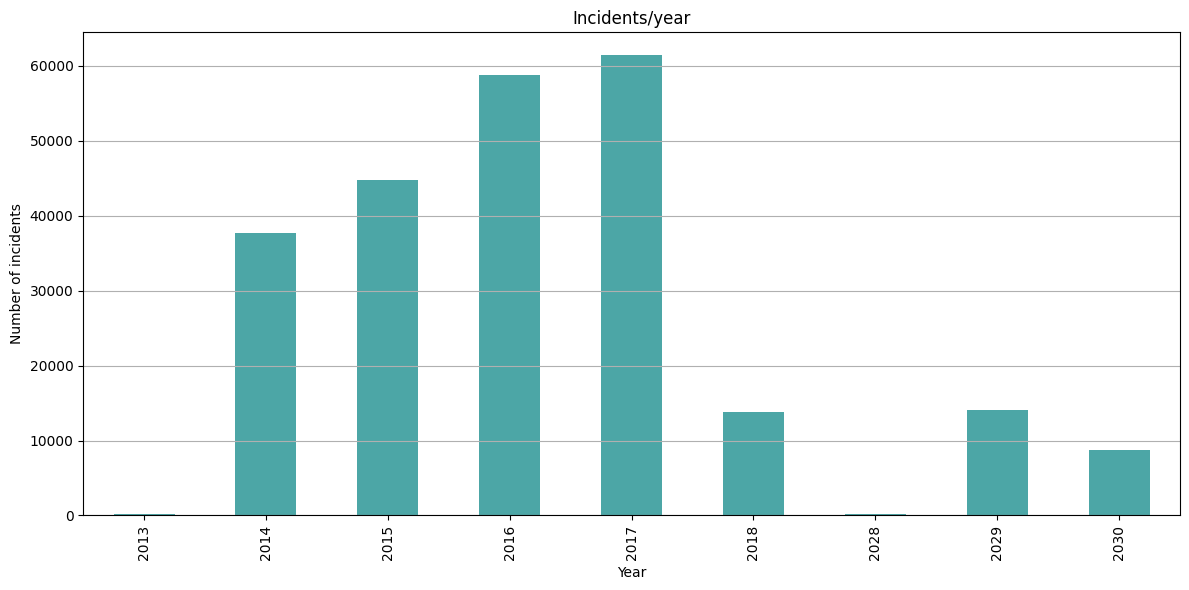
\includegraphics[width=0.8\textwidth]{incidents_per_year}
	\centering
	\caption{Number of incidents per year.}
	\label{incidents_per_year}
\end{figure}

\subsubsection{Geographical information}

The \textit{state} attribute contains no null values and it has 51 unique values: the 50 states of the United States and the District of Columbia, which we will consider as a special state.
Figure \ref{incidents_per_state} shows the number of incidents recorded in each state in decreasing order.

\begin{figure}[h]
	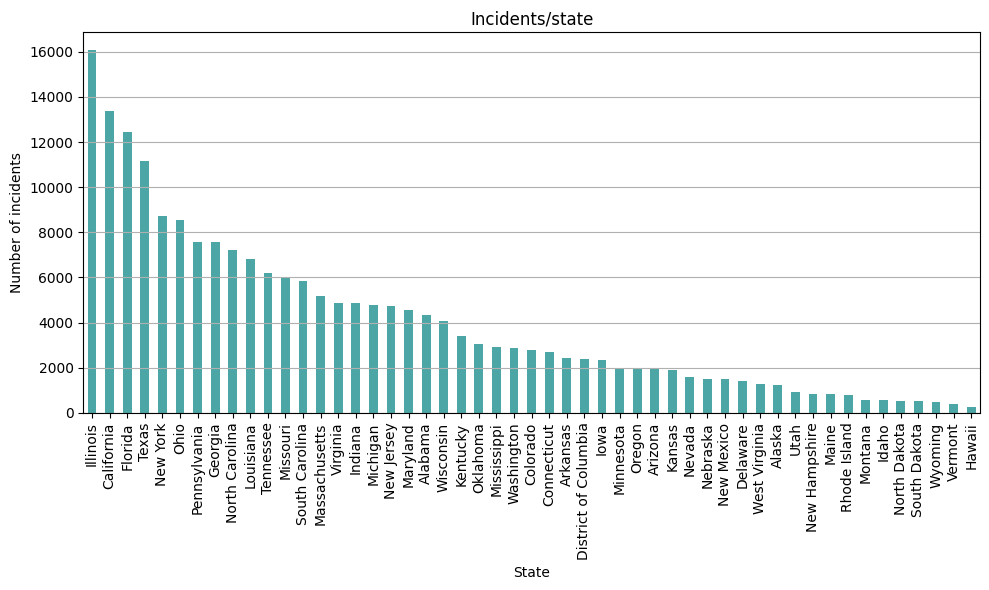
\includegraphics[width=0.8\textwidth]{incidents_per_state}
	\centering
	\caption{Number of incidents per state.}
	\label{incidents_per_state}
\end{figure}

The \textit{city\_or\_county} attribute has no null values, but it often contains additional informations about the suburb or the neighborhood in brackets, that provide a more precise location for the incident, e.g. ``Minneapolis (Brooklyn Center)".
%We consider removing this kind of information in the next phase.
%There are also instances containing the substring ``(county)" at the end, e.g. ``Orange (county)", that also appears as ``Orange": these instances will be substituted using just the name of the city/county.
Figure \ref{incidents_per_citycounty} shows the number of incidents recorded in each city/county in decreasing order.
\begin{figure}[H]
	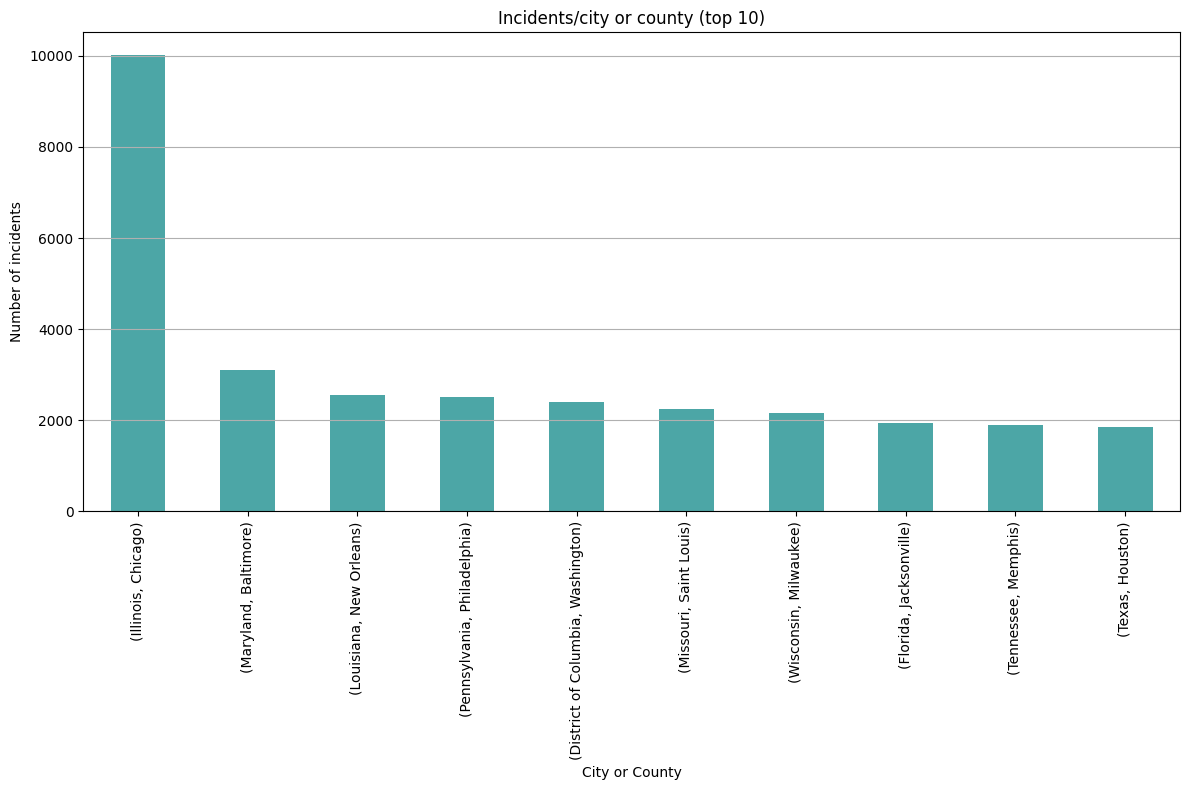
\includegraphics[width=0.8\textwidth]{incidents_per_citycounty}
	\centering
	\caption{Number of incidents per city or county.}
	\label{incidents_per_citycounty}
\end{figure}

The \textit{address} attribute contains some null values, but we believe it does not hold any statistical value, given that more specific information about the exact location of an incident is found by using the geographical coordinates.
Furthermore, there are only 6020 records for which address information can not be inferred using \textit{latitude} and \textit{longitude} attributes, so we will remove this column.

The \textit{latitude} and \textit{longitude} attributes contain some null values.
We also noticed some outliers by drawing empirical box boundaries of the United States: there are some incidents recorded outside of the U.S. that will be removed in the next phase.

Attributes \textit{congressional\_district}, \textit{state\_house\_district} and \textit{state\_senate\_district} contain some null values.
We also noticed that most of the incidents happened in the state of Illinois, by plotting the top 10 incidents for each of these attributes.

\subsubsection{Age and gender information}

The \textit{participant\_age1} attribute contains some outliers, mostly being values of type string and values that are too large to be the age of a person.
There are also some outliers if this attribute is compared to the corresponding value reported in the \textit{participant\_age\_group1} field.
As shown in Figure \ref{incidents_per_agegender}, most of the participants are adult males.
The attributes \textit{participant\_age1}, \textit{min\_age\_participants}, \textit{max\_age\_participants} and \textit{avg\_age\_participants} all have similar distributions.

The attributes \textit{n\_participants\_child}, \textit{n\_participants\_teen} and \textit{n\_participants\_adult} all present the same issues: they all contain outliers given by non-numerical strings, very large or negative numbers.

\begin{figure}[H]
	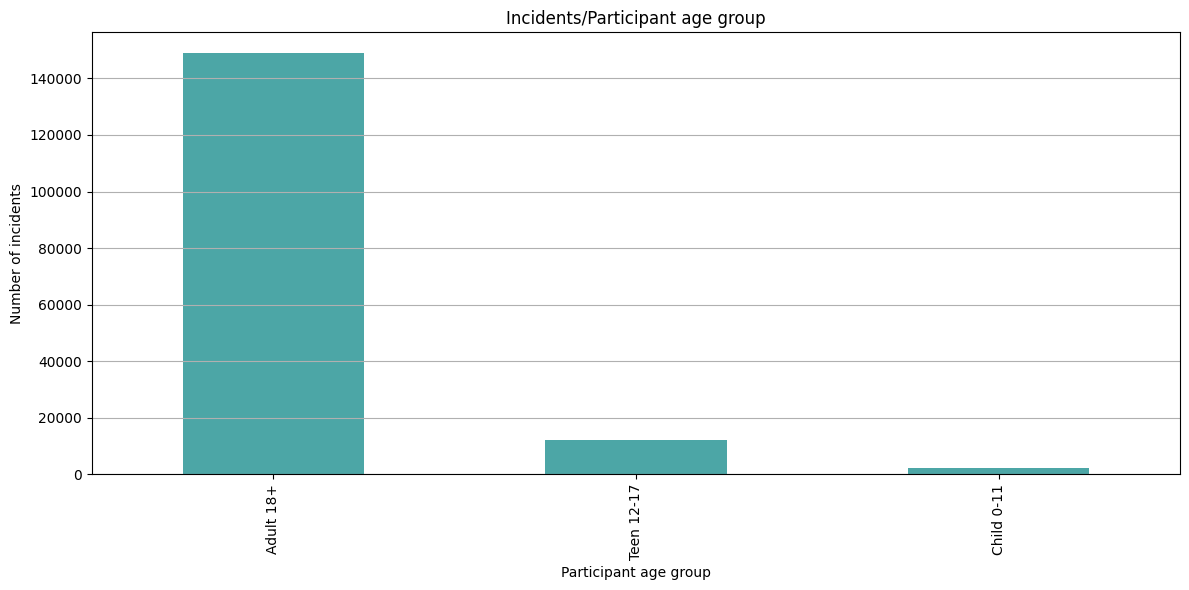
\includegraphics[width=0.8\textwidth]{incidents_per_agegroup}
	\centering
	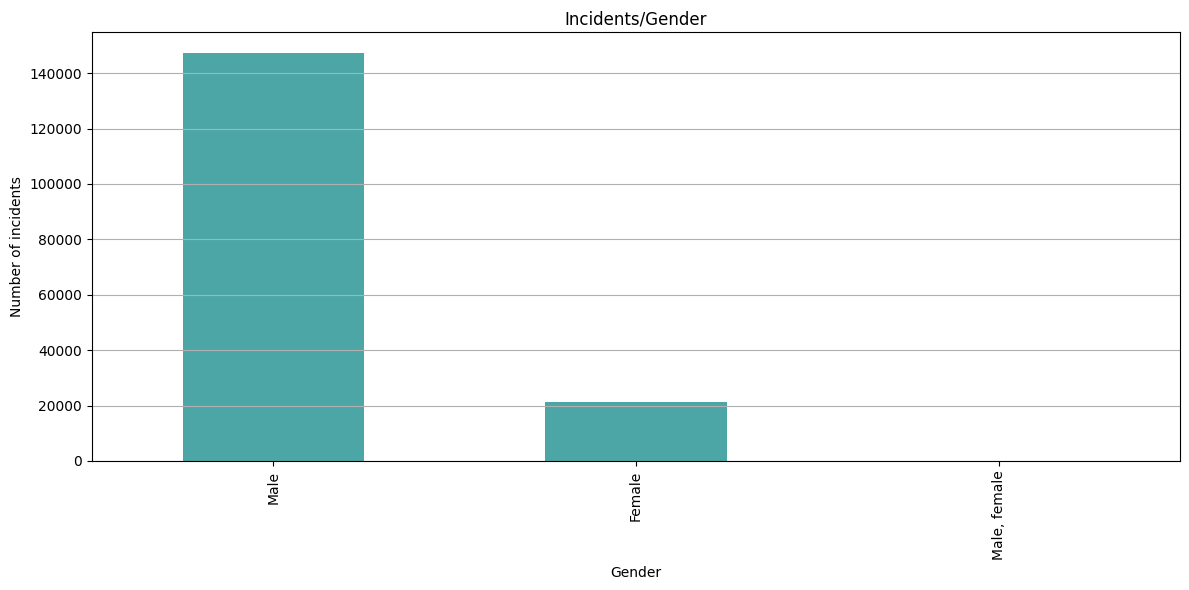
\includegraphics[width=0.8\textwidth]{incidents_per_gender}
	\caption{Number of incidents per age group (above) and gender (below) of the randomly chosen participant.}
	\label{incidents_per_agegender}
\end{figure}

\subsubsection{Number of involved people}

The majority of the incidents only involve between 0 and 5 people, with almost no killed, injured, unharmed or arrested people.

\subsubsection{Notes and incident characteristics}

We consider these attributes to hold no statistical value.

\subsection{Poverty by state}

The \textit{state} attribute contains 52 unique values: 51 of them are the same as the states in the incidents dataset, the remaining one is labeled ``United States" and contains the average of the whole country.
We consider using the average to possibly fill the missing values in the following phase.

There are no \textit{povertyPercentage} values for the year 2012, but we are only interested in relating this information to the incidents dataset, which only contains relevant incidents in the range of years 2013-2018.

\subsection{Year state district house}

This dataset contains no null values.
We will only consider data in the range of years 2013-2018 for integrating this data with the incidents dataset.

\section{Data Integration}

We created an additional column called \textit{total\_votes\_for\_state} in the year-state-house-district dataset: this column contains the total number of votes for each state and for each year.
We merged the incidents dataset with the poverty dataset using the attributes \textit{state} and \textit{year}.
We then merged the resulting dataset with the remaining one using the attributes \textit{state}, \textit{year} and \textit{congressional\_district}.
During the data integration process, records containing incidents set outside the U.S. were automatically deleted, resulting in a dataset that has no outliers in attributes \textit{latitude} and \textit{longitude}.
The dataset obtained by data integration will be used to further analyze and relate political party and poverty percentage to each congressional district.

\section{Distribution Analysis}

In order to analyze the features in the dataset, we displayed and examined the distribution of each column.
Figure \ref{age_du} shows the plots related to age attributes: as previously said, they all have very similar distributions.

\begin{figure}[h]
	\centering
	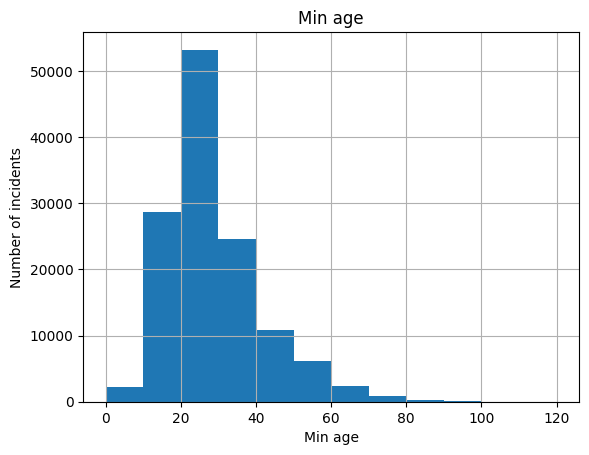
\includegraphics[width=0.5\textwidth]{min_age_du}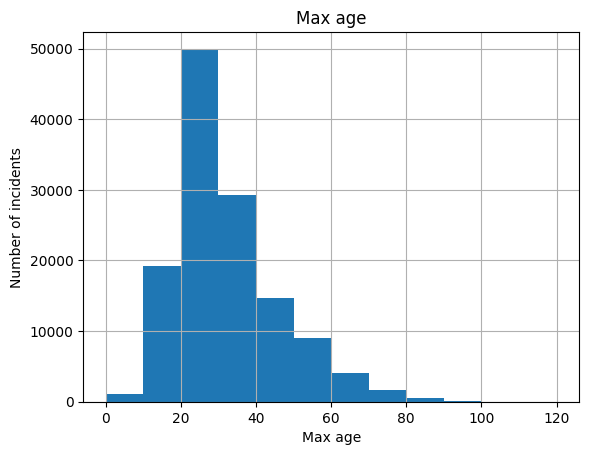
\includegraphics[width=0.5\textwidth]{max_age_du}
	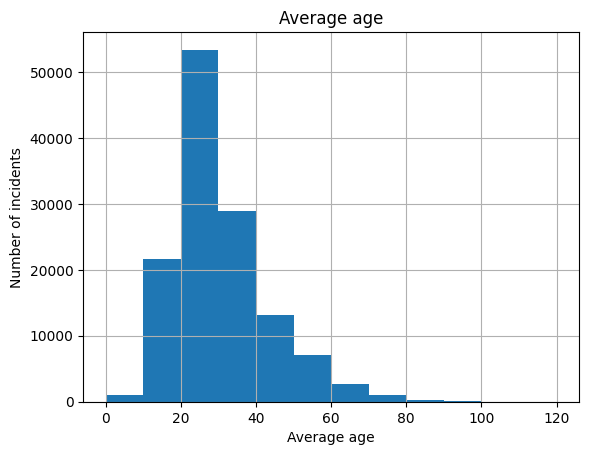
\includegraphics[width=0.5\textwidth]{avg_age_du}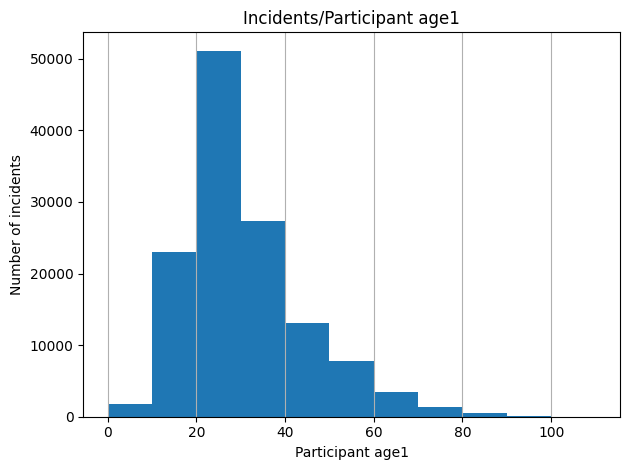
\includegraphics[width=0.5\textwidth]{part_age_du}
	\caption{Plot of minimum (top left), maximum (top right), average (bottom left) and participant1 (bottom right) age distributions.}
	\label{age_du}
\end{figure}

From Figure \ref{incidents_per_nparticipants} we can see that most of the incidents involve very few participants.
Specifically, the majority of them only involve between 0 and 3 participants, with incidents having only one person involved being the most common ones.

\begin{figure}[h]
	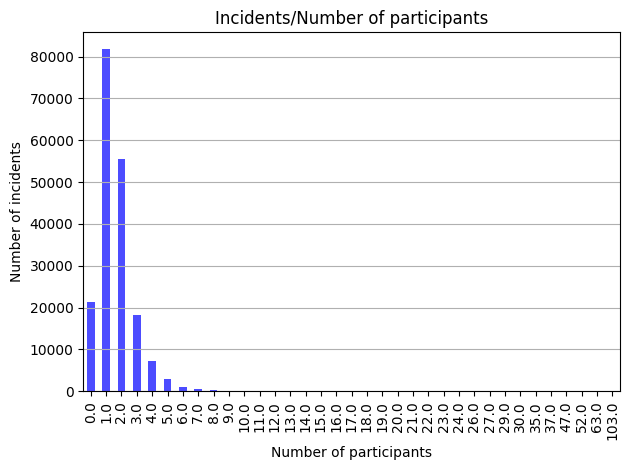
\includegraphics[width=0.6\textwidth]{incidents_per_nparticipants}
	\centering
	\caption{Number of incidents per number of people involved.}
	\label{incidents_per_nparticipants}
\end{figure}

As previously shown in Figure \ref{incidents_per_agegender}, the majority of participants recorded in the incidents is comprised of adult (18 years old or older) and male people.

\textbf{TODO} \textit{aggiungere gli screen dei plot delle mappe, quella degli shooting e quella dei mass shooting. in questo momento però non riesco a fare gli screen}\\
We also analyzed the geographical distribution of the incidents over the U.S. territory.
Specifically we focused on the number of killed people in each incidents in order to possibly understand the relation between killed people and geographical location.
The plots in Figure \ref{map_du} show the individual incidents recorded and the mass shooting events.
The incidents that resulted in 0 to 5 killed people are the majority, so the first map does not hold much meaning, given that most of the dots are records that report no killed people.
The second plot instead highlights events that are to be considered mass shootings and it shows some major events like, for example, Orlando (Florida) mass shooting in 2016 (50 killed people) and Southerland Springs (Texas) mass shooting (27 killed people).

\begin{figure}[h]
	\centering
	% TODO
	%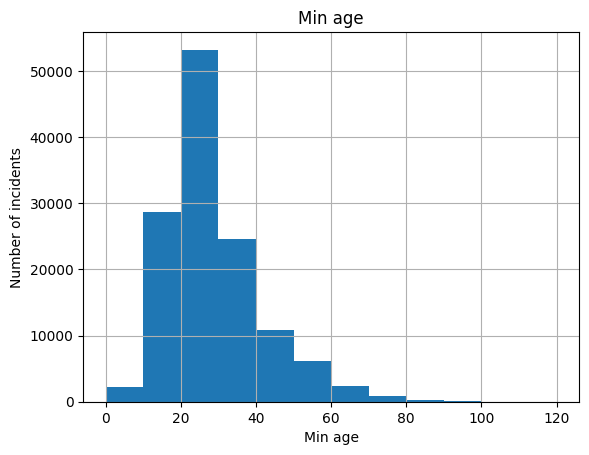
\includegraphics[width=0.5\textwidth]{min_age_du}\includegraphics[width=0.5\textwidth]{map_shooting}
	%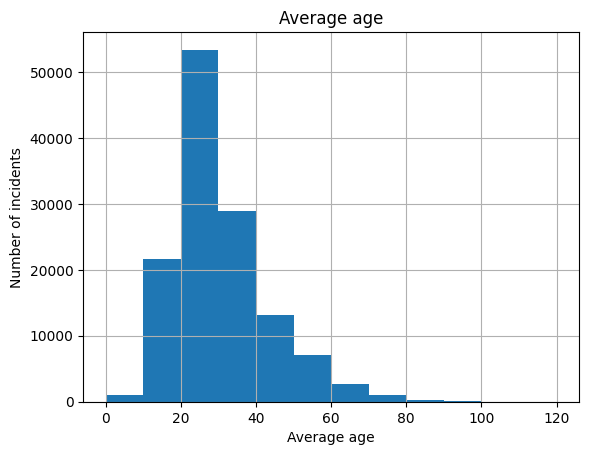
\includegraphics[width=0.5\textwidth]{avg_age_du}\includegraphics[width=0.5\textwidth]{map_massshooting}
	\caption{Map representing each incident (left) and mass-shooting incidents (right) recorded, the color used for the representation varies in relation to the number of people killed in the incident.
	The FBI has not set a minimum number of casualties to qualify an event as a mass shooting, but U.S. statute (the Investigative Assistance for Violent Crimes Act of 2012) defines a ``mass killing" as ``3 or more killings in a single incident." (\href{https://www.britannica.com/topic/mass-shooting}{source})}
	\label{map_du}
\end{figure}

\section{Correlation Analysis}

The correlation matrix is shown in Figure \ref{corr_matrix_du}.
At first glance, the only noteworthy correlations are those between the \textit{participant\_age1} feature of the randomly taken person and the attributes \textit{min\_age\_participants}, \textit{max\_age\_participants} and \textit{age\_age\_participants}.
This correlation is confirmed by the fact that the majority of the incidents only involve 1 or 2 participants. 
The correlation matrix will be computed again once outliers in the numerical attributes, which compromise the correlation calculation, have been eliminated.

We also observed that the number of males involved has a high correlation (0.83) with the number of participants because on average, as seen above, incidents tend to have a much more higher number of males participants than females participants.

\begin{figure}[h]
	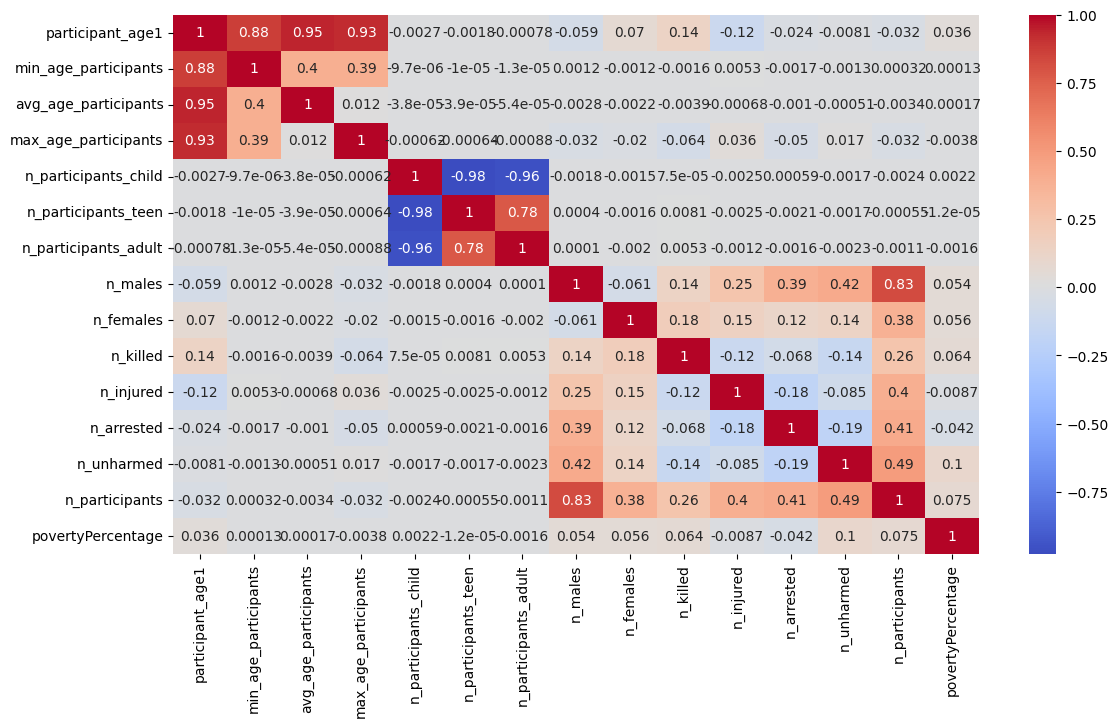
\includegraphics[width=1\textwidth]{corr_matrix_du}
	\centering
	\caption{Correlation matrix of numerical attributes.}
	\label{corr_matrix_du}
\end{figure}


\chapter{Data Preparation}

The data preparation phase uses the information gained in the previous phase to select records, manage outliers and missing values and improve data quality.
Each attribute was casted to the correct data type, in order to be coherent with the semantics of the feature, as shown in Table \ref{table01}.

\begin{table}[t]
	\centering
	\begin{small}
	\begin{tabular}{|l|l|l|p{7.7cm}|}
		\hline
		\textbf{Feature Name} & \textbf{Initial Type} & \textbf{Cast Type} & \textbf{Description}\\
		\hline
		date & object & Datetime64 & date of incident occurrence\\
		\hline
		state & object & String & state where incident took place\\
		\hline
		city\_or\_county & object & String & city or county where incident took place\\
		\hline
		address & object & String & address where incident took place\\
		\hline
		latitude & float64 & float64 & latitude of the incident\\
		\hline
		longitude & float64 & float64 & longitude of the incident\\
		\hline
		congressional\_district & int64 & Int64 & congressional district where the incident took place\\
		\hline
		state\_house\_district & int64 & Int64 & state house district\\
		\hline
		state\_senate\_district & float64 & Int64 & state senate district where the incident took place\\
		\hline
		participant\_age1 & float64 & Int64 & exact age of one (randomly chosen) participant in the incident\\
		\hline
		participant\_age\_group1 & object & String & exact age group of one (randomly chosen) participant in the incident\\
		\hline
		participant\_gender1 & object & String & exact gender of one (randomly chosen) participant in the incident\\
		\hline
		min\_age\_participants & object & Int64 & minimum age of the participants in the incident\\
		\hline
		avg\_age\_participants & object & float64 & average age of the participants in the incident\\
		\hline
		max\_age\_participants & object & Int64 & maximum age of the participants in the incident\\
		\hline
		n\_participants\_child & object & Int64 & number of child participants 0-11\\
		\hline
		n\_participants\_teen & object & Int64 & number of teen participants 12-17\\
		\hline
		n\_participants\_adult & object & Int64 & number of adult participants (18 +)\\
		\hline
		n\_males & float64 & Int64 & number of males participants\\
		\hline
		n\_females & float64 & Int64 & number of females participants\\
		\hline
		n\_killed & int64 & Int64 & number of people killed\\
		\hline
		n\_injured & int64 & Int64 & number of people injured\\
		\hline
		n\_arrested & float64 & Int64 & number of arrested participants\\
		\hline
		n\_unharmed & float64 & Int64 & number of unharmed participants\\
		\hline
		n\_participants & float64 & Int64 & number of participants in the incident\\
		\hline
		notes & object & String & additional notes about the incident\\
		\hline
		incident\_characteristics1 & object & String & incident characteristics\\
		\hline
		incident\_characteristics2 & object & String & incident characteristics\\
		\hline
		year & int64 & Int64 & year of the incident occurrence\\
		\hline
		povertyPercentage & float64 & float64 & poverty percentage for the corresponding state and year\\
		\hline
		party & object & String & winning party for the corresponding congressional\_district in the state, in the corresponding year\\
		\hline
		candidateVotes & int64 & Int64 & number of votes obtained by the winning party in the corresponding election\\
		\hline
		totalVotes & int64 & Int64 & total number of votes for the corresponding election\\
		\hline
		total\_votes\_for\_state & int64 & Int64 & total number of votes for each year and for each state\\
		\hline
	\end{tabular}
	\end{small}
	\caption{Features of the merged dataset}
	\label{table01}
\end{table}

Duplicate records and records where all null attributes where deleted.
For all numerical attributes, negative values were set to NaN.

\subsubsection{Date}

All records relating to events happened after 2023-10-01 (the date we received the dataset) were considered to be outliers, specifically to be errors in the data, and as such they were dropped.
We also dropped all records related to year 2013, as the year was under-represented.

\subsubsection{Age attributes}

For the attributes \textit{participant\_age1}, \textit{min\_age\_participants}, \textit{max\_age\_participants} and \textit{avg\_age\_participants}, values greater than or equal to 120 were considered to be outliers and set to NaN.
These three attributes seem to be very correlated, so we consider deleting the columns \textit{min\_age\_participants} and \textit{max\_age\_participants} and only keeping \textit{avg\_age\_participants}.
A further motivation for deleting these columns is that \textit{avg\_age\_participants} can not be inferred by computing the mean of min and max age attributes: when the average age is 0 or null, min and max age are also 0 or null.

\subsubsection{Geographical attributes}

The records with coordinates outside U.S. (other that null values) were automatically deleted after the data integration.
We consider the triple \textit{$<$date,latitude,longitude$>$} to be a key identifying an incident in a unique way: we assume that there are no incidents happening on the same day in the exact same geographic coordinates.
Hence, we decided to eliminate the records in which these 3 values are duplicates.
For the rows in which \textit{latitude} and \textit{longitude} are NaN, the missing values were filled using the mean computed for the corresponding \textit{state} and \textit{city\_or\_county}.
This allowed us to replace all missing values for \textit{latitude} and \textit{longitude}.

The columns \textit{state\_house\_district} and \textit{state\_senate\_district} were dropped from the dataset, given that they represent further subdivisions of the US territory that are not pertinent to our analysis.
In fact, we are only interested in the \textit{congressional\_district} data, because the electoral information provided has the same granularity.

\subsubsection{Number of participants attributes}

Outliers values found in \textit{n\_participants\_adult}, \textit{n\_participants\_teen} and \textit{n\_participants\_child} features, namely those due to enormous values, were set to NaN.
In particular, they were set to NaN when their value exceeded the maximum value found in column \textit{n\_participants} (which has no significant large values).
Furthermore, in records that had \textit{n\_participants} equal to 0, the attributes relating to the number of participants were also set to 0.

In order to keep the dataset coherent, the value in \textit{n\_participants} was replaced with the sum \textit{n\_males} + \textit{n\_females}, if this sum is equal to (\textit{n\_participants\_adult} + \textit{n\_participants\_teen} + \textit{n\_participants\_child}) and different from \textit{n\_participants}.
Viceversa, we set to NaN these attributes in the rows where these sums and/or \textit{n\_participants} are not equal.
The NaN values were then substituted using the mean of each attribute, grouped by \textit{n\_participants}; the few (8) rows for which this replacement was not possible (we were not able to reconstruct the mean) were dropped from the dataset.
There were no relevant changes in the distribution of these attributes after the cleaning.

We checked whether the number of killed, injured, arrested and unharmed people exceeds the total number of participants in that incident.
In case they do, we set them to NaN and then proceeded to fill null values using the mean.
There was no major change in the distribution of these feature after this operation.

\subsubsection{Incident characteristics}

In order to fill the missing values for feature \textit{incident\_characteristics1}, records were analyzed by looking at data from \textit{n\_killed}, \textit{n\_injured} and \textit{notes} attributes.
This was done to create subgroups of records, so that incidents characteristics could be reconstructed if missing.
For records that did not fit in any of these subgroups, \textit{incident\_characteristics1} was filled using the string ``Shots Fired - No Injuries", as they reported no injured or killed people.
We dropped the column \textit{incident\_characteristics2} given that it has 40\% of null values and does not add meaningful details for our analysis.

\section{Correlation analysis}

The correlation matrix, shown in Figure \ref{corr_matrix_dp}, has been computed only for numerical attributes.
It can be seen that age attributes are highly correlated.
Because of this, we decided to drop all of them\footnote{We dropped \textit{participant\_age1}, \textit{min\_age\_participants} and \textit{max\_age\_participants}.} except for \textit{avg\_age\_participants}, which is the most correlated ($>90\%$) to the other attributes and gives us more general informations about all the participants.
Given the fact that \textit{participant\_age1} was dropped, the attributes \textit{participant\_gender1} and \textit{participant\_age\_group1} become useless because there no longer is any information about the randomly selected person: they were also dropped.
The only remaining feature related to the participants age is \textit{avg\_age\_participants}, which contains some null values.
The missing values filled by the mean, by considering the number of adults, teens and children involved in the incident.

It can also be noticed that \textit{n\_participants\_adult} and \textit{n\_males} are highly correlated.
Furthermore, they can both be obtained by mean of sums of other attributes\footnote{In particular,
$n\_participants = n\_participants\_adult + n\_participants\_teen + n\_participants\_child$, but also $n\_participants = n\_males + n\_females$.
All attributes relating to the number of participants were dropped, with the excepytion of \textit{n\_participants}, which conveys the most general information.}, so they were dropped.

We also decided to drop the columns \textit{year} (just a result of data integration), \textit{address} and \textit{notes}.

\begin{figure}[h]
	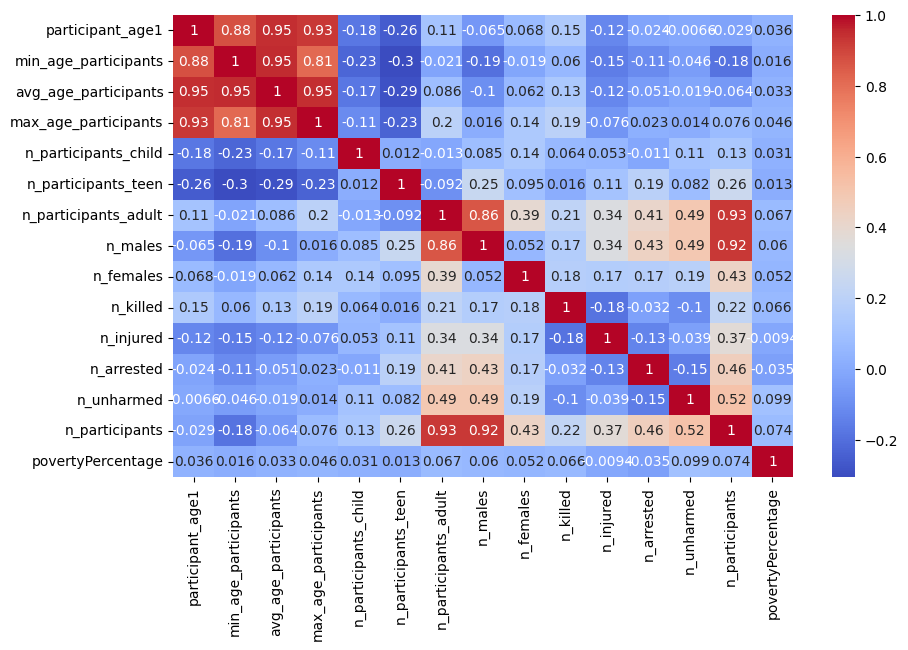
\includegraphics[width=0.8\textwidth]{corr_matrix_dp}
	\centering
	\caption{Correlation matrix of numerical attributes.}
	\label{corr_matrix_dp}
\end{figure}

\section{Definition of indicators}

After analyzing the data, we considered the following indicators as being representative of an incident severity:
\begin{itemize}
	\item \textit{incident\_gravity}, number of killed and injured people in an incident,
	\item \textit{females\_rate}, number female people involved in the incident over the total number of participants in that incident,
	\item \textit{minor\_rate}, number minors (younger than 17 years old) involved in the incident over the total number of participants,
	\item \textit{arrested\_rate}, number arrested people in the incident over the total number of participants,
	\item \textit{survival\_rate}, number unharmed people in the incident over the total number of participants,
	\item \textit{injured\_rate}, number injured people in the incident over the total number of participants,
	\item \textit{killed\_rate}, number killed people in the incident over the total number of participants,
	\item \textit{winning\_party\_percentage}, the number of votes for the winning candidate over the total number of votes in that election.
	\item \textit{killed\_disp\_per\_district}, number of killed people in the incident over the number of killed people in that same congressional district in the same year,
	\item \textit{injured\_disp\_per\_district}, number of injured people in the incident over the number of injured people in that same congressional district in the same year,
	\item \textit{part\_disp\_per\_district}, number of participants in the incident over the number of participants in incidents in that same congressional district in the same year.
\end{itemize}

The correlation matrix of the chosen indicators is the one in Figure \ref{corr_matrix_indicators}.
Indicators \textit{female\_ratio} and \textit{minor\_ratio} both have similar behaviors and distributions.
For most of the incidents, the rates of survival, arrested, injured and killed people are equal to 0.
A lot of incidents involving injuries, arrests or survivors do not involve deaths.
Similarly, incidents involving injuries, arrests or deaths do not involve any survivors.
Indicators \textit{arrested\_rate} and \textit{injured\_rate} have a similar behavior.
This confirms that these indicators are uncorrelated. 
\begin{figure}[h]
	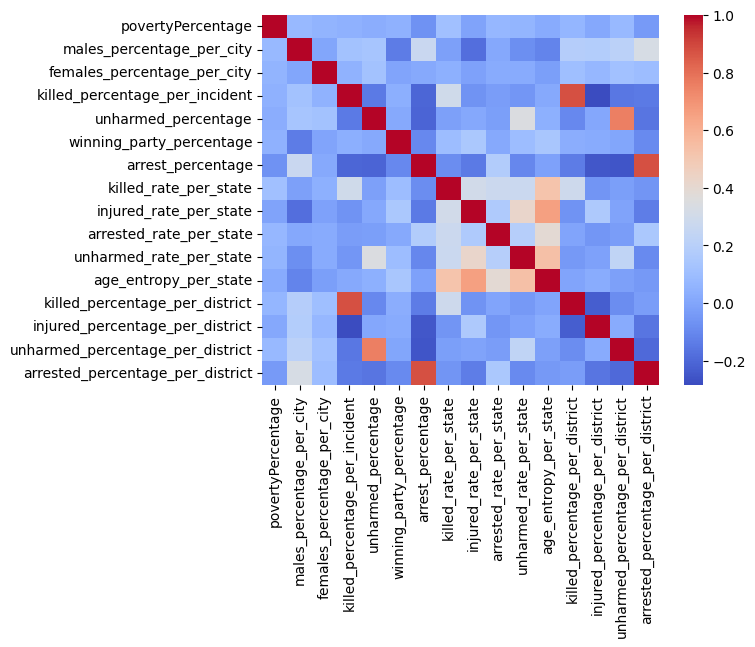
\includegraphics[width=1\textwidth]{corr_matrix_indicators}
	\centering
	\caption{Correlation matrix plotted of the newly created indicators}
	\label{corr_matrix_indicators}
\end{figure}

The last three indicators often have value 0, which is also the value of the mean.
Over all, the indicators we identified have no missing values; they have some outliers that are coherent with the one in the numerical attributes, so we decided not to clean them.
All these indicators provide a good characterization of the incidents and are at most moderately correlated.

\chapter{Clustering}

\section{Preprocessing}

In order to apply clustering methods, data needs to be prepared through some steps of preprocessing.
First of all some new binary columns were added and used to label the PCA results:
\begin{itemize}
	\item \textit{involve\_killing}, its value is 0 if nobody was killed in the incident, it is 1 if at least a person was killed;
	\item \textit{involve\_injury}, its value is 0 if nobody was injured in the incident, it is 1 if at least a person was injured;
	\item \textit{involve\_arrest}, its value is 0 if nobody was arrested in the incident, it is 1 if at least a person was arrested;
	\item \textit{is\_survived}, its value is 0 if nobody survived in the incident, it is 1 if at least a person survived.
\end{itemize}
The new feature \textit{involve\_killing} will also be used in the following classification task.
Given that for clustering we will use a distance metric, that only works on numerical attributes, we remove categorical attributes for this task and we only use the indicators listed in the previous section.
The features are also normalized: scaling data is useful to avoid some values being too large and prevailing on the others when a clustering algorithm is applied, so we computed a normalization of the numerical values.

The Principal Component Analysis is computed using two components.
It yields a 2-dimensional visualization of the multidimensional data considered, shown in Figure \ref{pca}.

\begin{figure}[h]
	\centering
	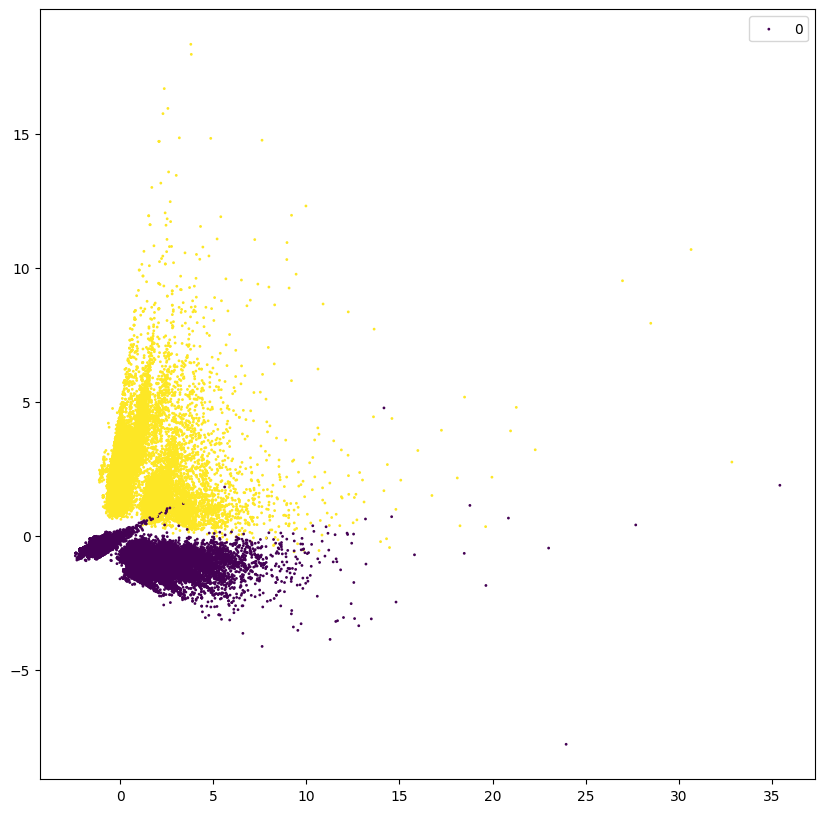
\includegraphics[width=0.5\textwidth]{pca_killing}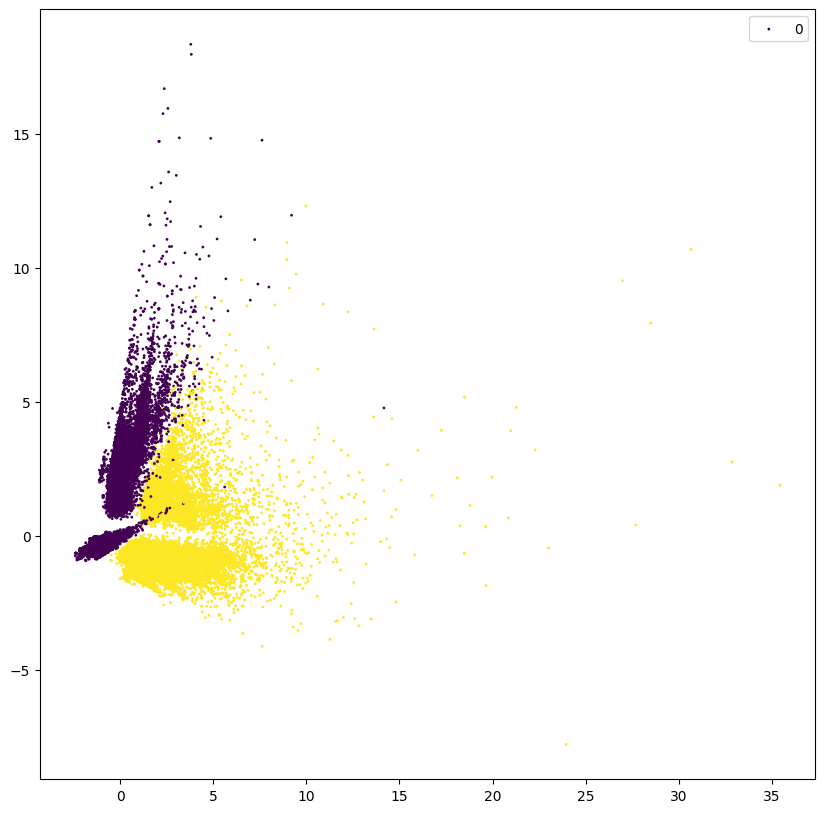
\includegraphics[width=0.5\textwidth]{pca_injury}
	\caption{PCA, with number of components equal to 2.
	The color of the points corresponds to the value of \textit{involve\_killing} in the left plot and to the value of \textit{involve\_injury} in the right plot.}
	\label{pca}
\end{figure}

\section{K-Means}

In order to estimate the best value of $k$ to then apply the K-means clustering algorithm, the elbow method was used.
The grid search on values of $k \in \{2, 3, 4, 10, 100, 100\}$ yielded the following results (Table \ref{table02}), evaluated in terms of the metrics SSE, separation and silhouette.
A plot of the SSE and silhouette scores is shown in Figure \ref{kmeans_k}.
\begin{table}[h]
	\centering
	\begin{small}
		\begin{tabular}{l|p{4cm}|p{4cm}|p{4cm}}
		\textbf{K} & \textbf{SSE} & \textbf{separation} & \textbf{silhouette}\\
		\hline
		2 & 1868436.1752223005 & 1.9881698493281088 & 0.1938016918423718\\
		3 & 1562300.2158580532 & 1.6287560855244605 & 0.24111879379810464\\
		4 & 1401333.0002367594 & 1.435772151754466 & 0.24457341442342728\\
		10 & 935031.5401451141 & 1.4857417427196573 & 0.27681666821740364\\
		100 & 315602.0491054469 & 1.3057093979420389 & 0.26549526914793403\\
		1000 & 96365.98745985169 & 1.2338707526266535 & 0.2938211523306092\\
	\end{tabular}
	\end{small}
	\caption{Values of SSE, separation and silhouette score computed for increasing values of $k$.}
	\label{table02}
\end{table}
\begin{figure}[h]
	\centering
	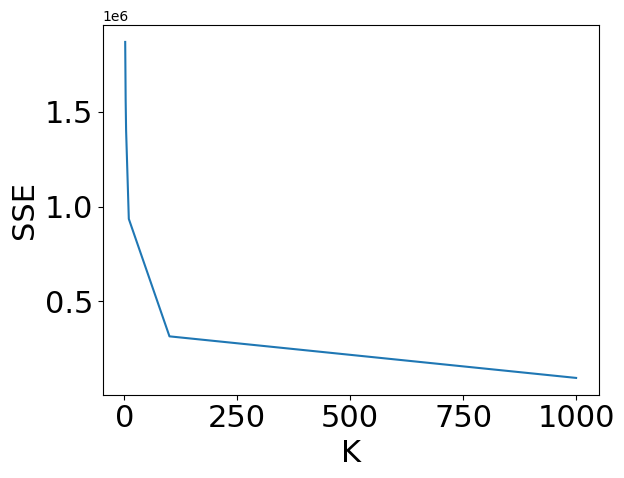
\includegraphics[width=0.35\textwidth]{kmeans_sse}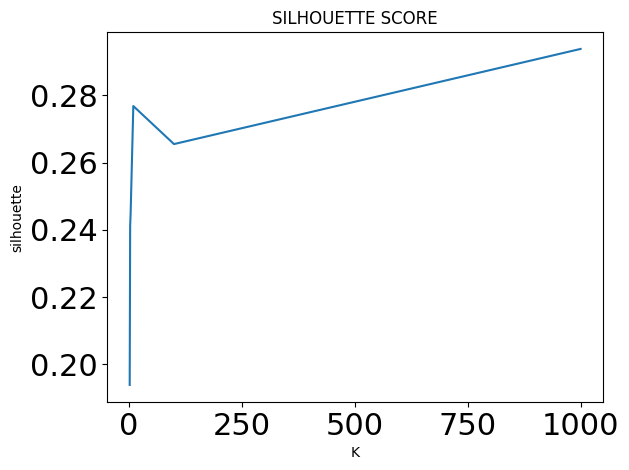
\includegraphics[width=0.35\textwidth]{kmeans_silhouette}
	\caption{Plots of SSE (left) and the silhouette (right) scores.}
	\label{kmeans_k}
\end{figure}

Both the elbow method and the silhouette score point out that the best value for $k$ is around 3.
After fitting the method to our data, the clustering results were plotted on the 2 PCA dimensions, label the points according to the belonging cluster.
The plot is shown in Figure \ref{kmeans_pca}, along with the cluster label distribution.
\begin{figure}[h]
	\centering
	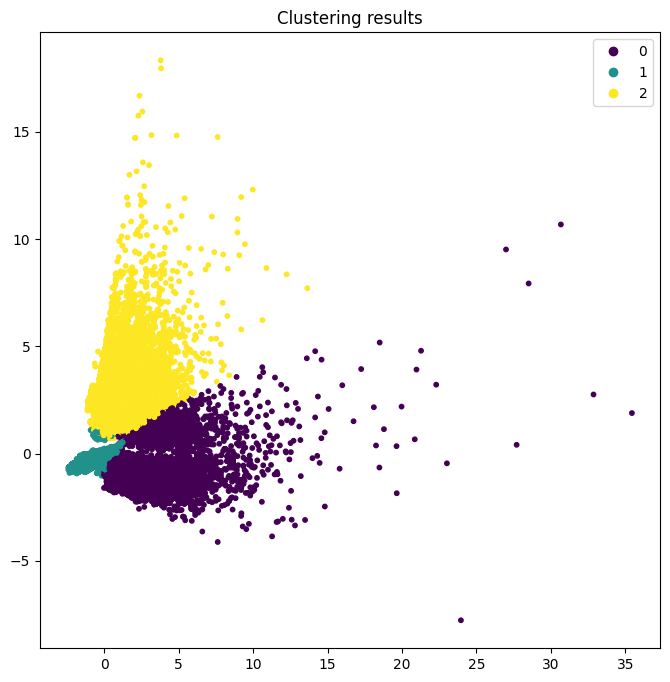
\includegraphics[width=0.4\textwidth]{kmeans_pca}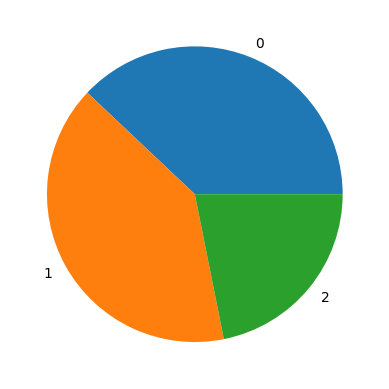
\includegraphics[width=0.35\textwidth]{kmeans_pie}
	\caption{Plots of the PCA components after the clustering labeling (left) and the distribution of the cluster labels (right).}
	\label{kmeans_pca}
\end{figure}

Figure \ref{kmeans_killing} shows the distribution of values of feature \textit{involve\_killing} in the three clusters found.
The first two clusters contain a majority of non fatal incidents, while the third cluster only contains incidents involving at least one killed person.
\begin{figure}[h]
	\centering
	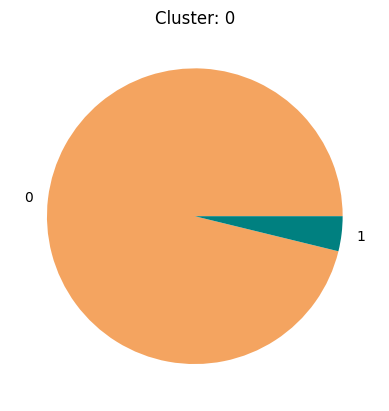
\includegraphics[width=0.2\textwidth]{kmeans_0}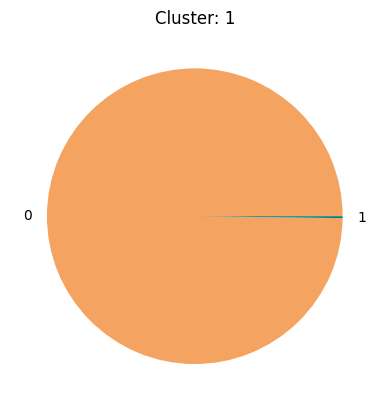
\includegraphics[width=0.2\textwidth]{kmeans_1}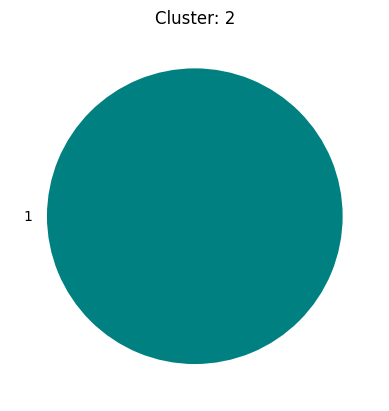
\includegraphics[width=0.2\textwidth]{kmeans_2}
	\caption{Plots of the three clusters found by applying K-means, labeled according to the value of \textit{involve\_killing}.
	Cluster 0 has 68459 incidents for which \textit{involve\_killing} is 0, 2714 incidents for which it is 1;
	Cluster 1 has 75225 incidents for which \textit{involve\_killing} is 0, 155 incidents for which it is 1;
	Cluster 2 contains 40981 incidents for which \textit{involve\_killing} is 1.}
	\label{kmeans_killing}
\end{figure}

\subsection{X-Means}

The X-means implementation used is \textit{pyclustering}\footnote{Pyclustering: \url{https://github.com/annoviko/pyclustering/}}.
The starting parameter for X-means was a maximum number of clusters of 10, repeating 10 times the execution of K-means, starting from 7 centroids.
Computing the clusters using the X-mean algorithm, the result was composed of 10 clusters.
The metrics of silhouette and separation obtained from these clusters were 1.4333188536330668 and 0.2239619283502909 respectively.
The distribution of values of feature \textit{involve\_killing} per cluster and the distribution of the cluster labels are shown in Figure \ref{xmeans_killing}.
It can be noticed that the distribution of the cluster labels is uneven.

\textbf{TODO:} \textit{inserire SSE!!}
\begin{figure}[h]
	\centering
	\begin{minipage}{0.75\textwidth}
		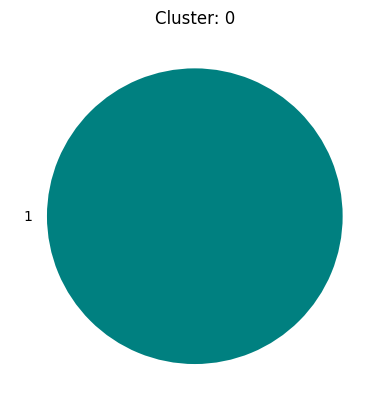
\includegraphics[width=0.2\textwidth]{xmeans_0}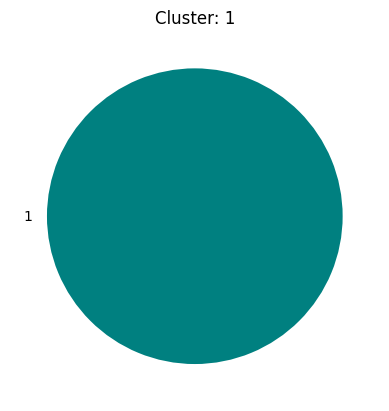
\includegraphics[width=0.2\textwidth]{xmeans_1}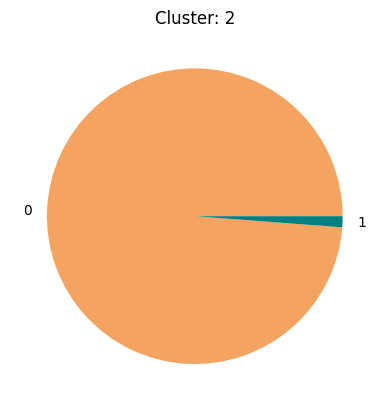
\includegraphics[width=0.2\textwidth]{xmeans_2}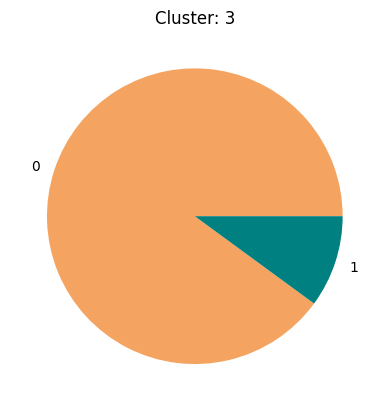
\includegraphics[width=0.2\textwidth]{xmeans_3}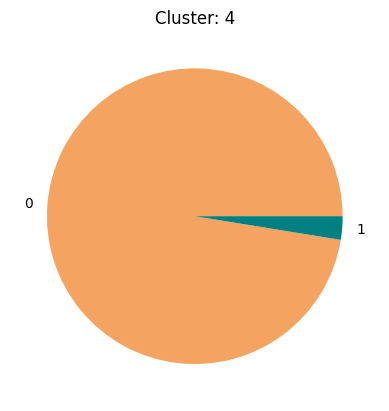
\includegraphics[width=0.2\textwidth]{xmeans_4}
		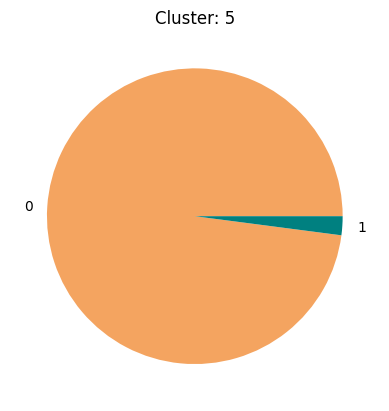
\includegraphics[width=0.2\textwidth]{xmeans_5}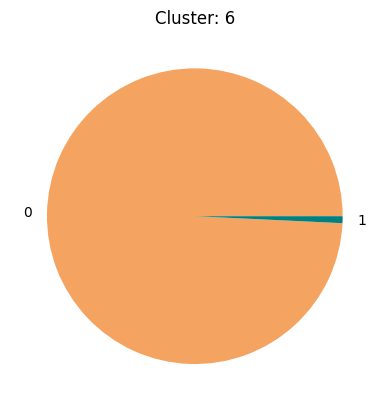
\includegraphics[width=0.2\textwidth]{xmeans_6}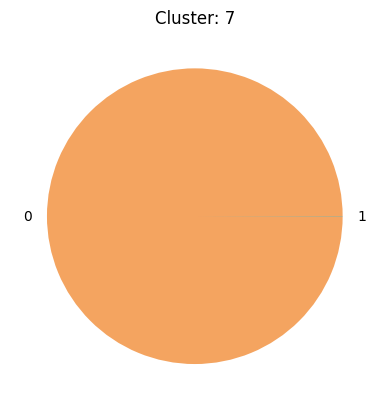
\includegraphics[width=0.2\textwidth]{xmeans_7}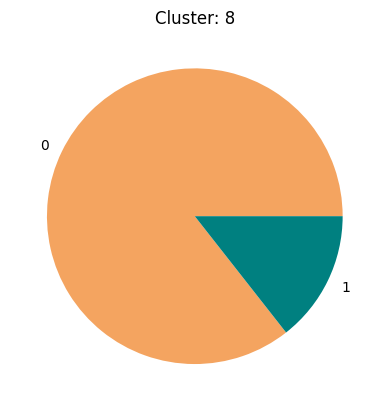
\includegraphics[width=0.2\textwidth]{xmeans_8}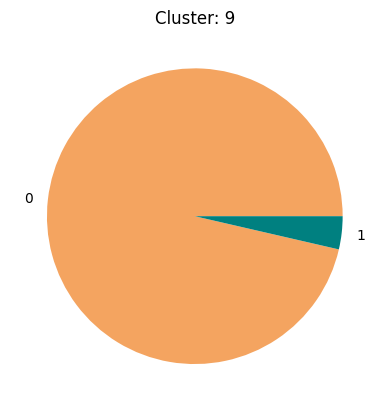
\includegraphics[width=0.2\textwidth]{xmeans_9}
	\end{minipage}%
	\begin{minipage}{0.25\textwidth}
		\centering
		\vspace{1cm}
		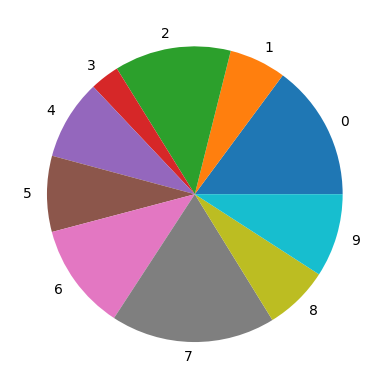
\includegraphics[width=1\textwidth]{xmeans_distribution}
		\vspace{0.8cm}
	\end{minipage}
		\caption{Plots of the ten clusters found applying X-means (left), labeled according to the value of \textit{involve\_killing}, and the plot of the distribution of the cluster labels (right).}
		\label{xmeans_killing}
\end{figure}

\section{Dbscan clustering}

As per the classification subtask in the project description, only one state was chosen for this clustering task: the state of Illinois, that is the first state per number of gun incidents (15319).
Density-based clustering algorithms are used to identify irregularly shaped clusters.
In order to estimate the best value for the epsilon ($\varepsilon$) parameter, the elbow method was used: computing the distance to the $k$ nearest neighbors and sorting them in decreasing order resulted in the plot shown in Figure \ref{dbscan_elbow}.
The best estimation found for the value of $\varepsilon$ is around 1.5.
Different values of $\varepsilon$ were then explored along with varying values of \textit{min\_samples}, resulting in Table \ref{table03}, shown in decreasing order of silhouette score.
Therefore, the best values of $\varepsilon$ and \textit{min\_samples} are 1.6 and 160 respectively.

Applying Dbscan to the dataset using the parameters listed above lead to finding 4 clusters.
Figure \ref{dbscan_elbow} also shows the scatter plot of these results on the 2 PCA components defined before, along with the distribution of the cluster labels.
The plots show that all the incidents in which there was at least a person killed belong to Cluster 2, while Clusters 0, 1 and 3 only feature non-deadly incidents.
\begin{table}[h]
	\centering
	\begin{small}
		\begin{tabular}{c|c|c|c|c}
			\textbf{$\varepsilon$} & \textbf{silhouette} & \textbf{DBscore} & \textbf{n\_clusters} & \textbf{min\_samples}\\
			\hline
			1.6 & 0.202494 & 001814 & 5 & 160\\
			1.6 & 0.199733 & 004573 & 5 & 170\\
			1.6 & 0.197965 & 998093 & 5 & 180\\
			1.7 & 0.180224 & 643053 & 3 & 180\\
			1.7 & 0.086065 & 570127 & 4 & 160\\
			1.7 & 0.073308 & 567566 & 4 & 170\\
	\end{tabular}
	\end{small}
	\caption{Table showing the search for the best values of $\varepsilon$ and \textit{min\_samples} parameters.}
	\label{table03}
\end{table}

\begin{figure}[h]
	\centering
	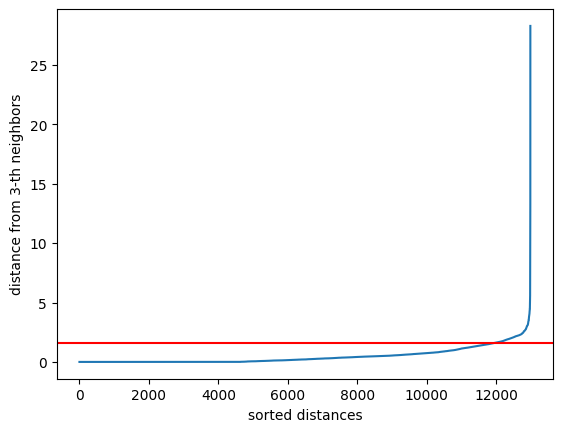
\includegraphics[width=0.4\textwidth]{dbscan_elbow}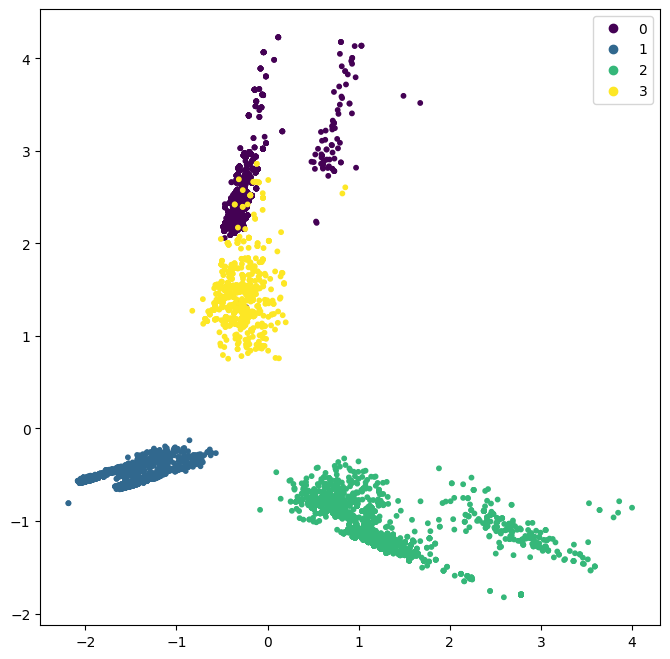
\includegraphics[width=0.31\textwidth]{dbscan_pca}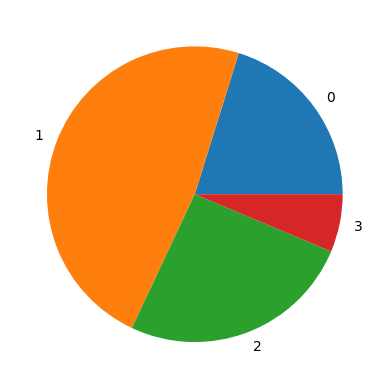
\includegraphics[width=0.3\textwidth]{dbscan_distribution}
	\caption{Plots of the elbow method result (left), the PCA components after the clutering labeling (middle) and the distribution of the cluster labels (right).}
	\label{dbscan_elbow}
\end{figure}

\begin{figure}[h]
	\centering
	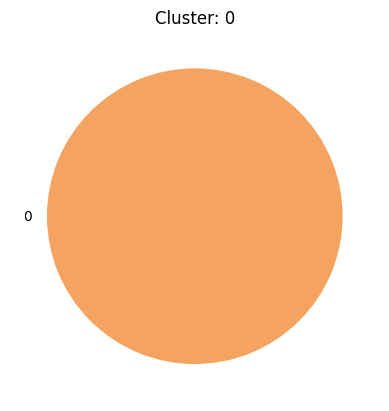
\includegraphics[width=0.2\textwidth]{dbscan_0}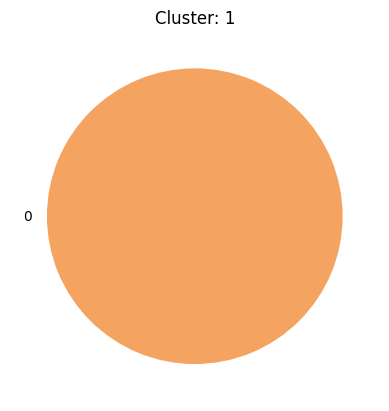
\includegraphics[width=0.2\textwidth]{dbscan_1}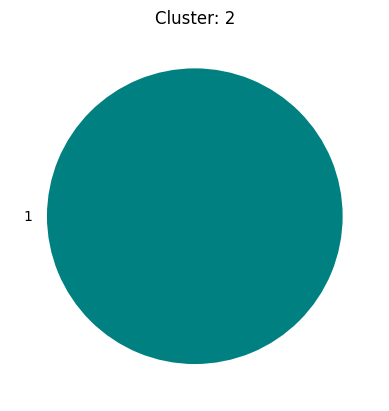
\includegraphics[width=0.2\textwidth]{dbscan_2}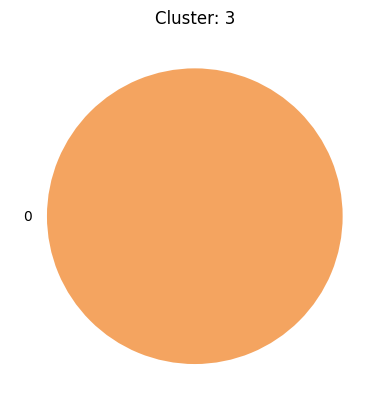
\includegraphics[width=0.2\textwidth]{dbscan_3}
	\caption{Plots of the four clusters found applying Dbscan, labeled according to the value of \textit{involve\_killing}.}
	\label{xmeans_killing}
\end{figure}

\section{Hierarchical clustering}

As per the classification subtask in the project description, only one state was chosen for this clustering task: the state of California, that is the second state per number of gun incidents (12980).
In order to identify the best metric for distance and the best method, we evaluated different trials.
The best results were obtained by using the correlation distance metric and the weighted linkage method.
The correlation distance between vectors $u$ and $v$ is defined as
$$1 - \frac{(u-\bar{u})\cdot(v-\bar{v})}{\left \Vert (u-\bar{u}) \right \|_2 \left \Vert (v-\bar{v}) \right \|_2},$$
where $\bar{v}$ is the mean of the elements of vector $v$.
The weighted linkage method, instead, assigns $$d(u,v) = \frac{dist(s,v)+dist(t,v)}{2},$$
where cluster $u$ was formed with cluster $s$ and $t$ and $v$ is a remaining cluster in the forest.

By using this final model, the silhouette score is 0.2589355057625014 and the DBscore 1.4509696821004128.
The dendrogram displayed in Figure \ref{hiera} was truncated at level 5, so that it can better be observed.
The cluster label distribution is not even: the cluster sizes are, in order, 772, 5018, 2697, 513, 3980.

\begin{figure}[h]
	\centering
	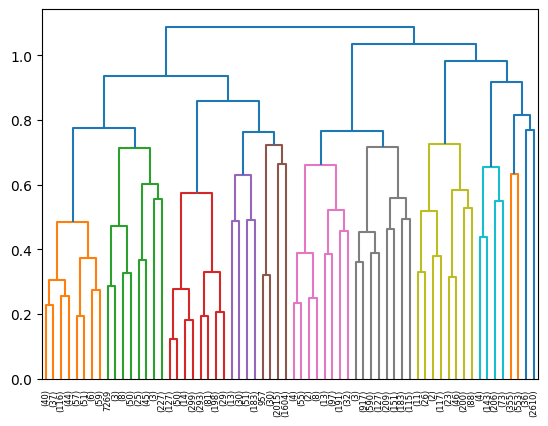
\includegraphics[width=0.5\textwidth]{hiera_dendro}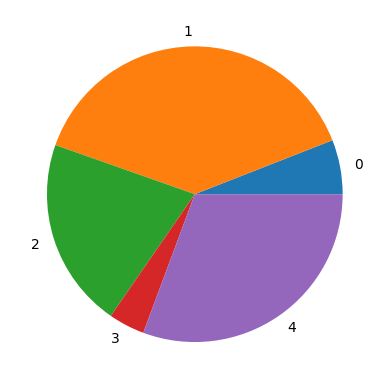
\includegraphics[width=0.4\textwidth]{hiera_distribution}
	\caption{Plots of the dendrogram obtained by applying Dbscan (left) and the distribution of the cluster labels (right).}
	\label{hiera}
\end{figure}

\begin{figure}[h]
	\centering
	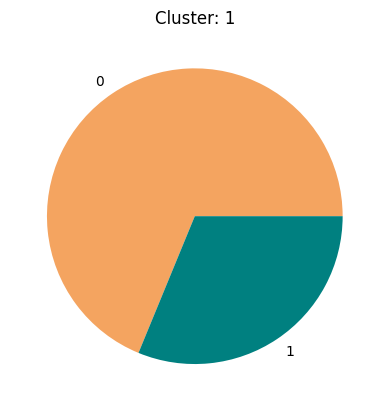
\includegraphics[width=0.2\textwidth]{hiera_1}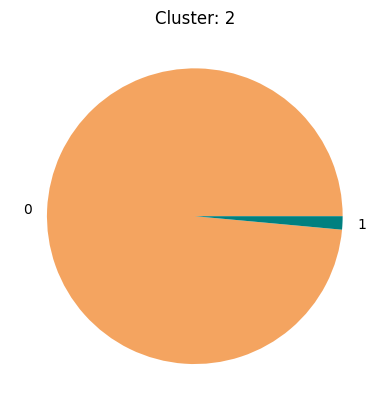
\includegraphics[width=0.2\textwidth]{hiera_2}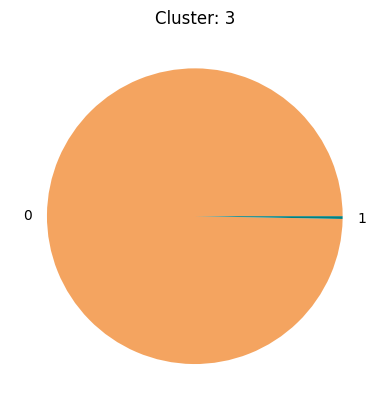
\includegraphics[width=0.2\textwidth]{hiera_3}\includegraphics[width=0.2\textwidth]{hiera_4}\includegraphics[width=0.2\textwidth]{hiera_5}
	\caption{Plots of the five clusters found applying agglomerative hierarchical clustering, labeled according to the value of \textit{involve\_killing}.}
	\label{hiera_killing}
\end{figure}

After applying all the methods shown before and analyzing the results obtained, we chose Dbscan as the best performing clustering algorithm, both because of the cluster distribution and the  distribution of records reporting at least one dead person in the incident.

\chapter{Classification}

\chapter{Explanation Analysis}

\end{document}
